\documentclass[10pt,letterpaper]{article}

\usepackage{cogsci}
\usepackage{pslatex}
\usepackage{apacite}
\usepackage{graphicx}
\usepackage{caption}
\usepackage{subfigure}
%\usepackage{subcaption}
\usepackage{subfigure}
\graphicspath{{figures/}}
  
\usepackage{color}

\definecolor{Red}{RGB}{255,0,0}
\newcommand{\red}[1]{\textcolor{Red}{#1}}  
  
\usepackage{listings}
%\usepackage{inconsolata}
\usepackage{xcolor} %to use colored text

%\lstset{
%language=Scheme,
%basicstyle=\footnotesize\ttfamily,
%mathescape=true,
%frame=single
%}

\lstset{
  language=Scheme, % Andreas Stuhlmüller. Scheme listings. https://github.com/stuhlmueller/scheme-listings.git
  columns=fixed,
  tabsize=2,
  extendedchars=true,
  breaklines=true,
  frame=single,
%  numbers=left,
  numbersep=5pt,
    basicstyle=\scriptsize\ttfamily
%  rulesepcolor=\color{solarized@base03},
%  numberstyle=\tiny\color{solarized@base01},
%  keywordstyle=\color{solarized@green},
%  stringstyle=\color{solarized@cyan}\ttfamily,
%  identifierstyle=\color{blue},
%  commentstyle=\color{solarized@base01},
%  emphstyle=\color{solarized@red}
}

\begin{document}

\title{Some arguments are probably valid: Reason and conversation in syllogisms}
 
\author{{\large \bf Michael H. Tessler, Noah D. Goodman } \\
	\{mtessler, ngoodman\}@stanford.edu \\
  Department of Psychology, Stanford University}

\maketitle


\begin{abstract}
We develop a computational-level theory of syllogistic reasoning which places reasoning at the intersection of communication and logic. We compare our model predictions with behavioral data from a recent meta-analysis. We show the flexibility of the model to account for reasoning behavior in a study of so-called ``statistical syllogisms" which use the generalized quantifiers \emph{most} and \emph{few}. We relate our model to three extant theories of syllogistic reasoning -- Mental Models, Mental Logics and Probability Heuristics. We conclude by discussing further predictions of the model and future directions.  
\\
\textbf{Keywords:} 
Reasoning, language understanding, probabilistic model
\end{abstract}


Consider for a moment that your friend tells you:
``Everyone in my office has the flu and, you know, some people with the flu are out for weeks.''
Do you respond with
``Everyone in your office has the flu.''
Do you respond with
``Pardon me, there is no inference I can draw from what you just said."
Or do you respond
 ``I hope your officemates are not out for weeks and I hope you don't get sick either."
 The first response is true, but does not go beyond the premises; the second response attempts to go beyond the premises by strict classical logic, but fails; the final response goes beyond the premises, to offer a conclusion which is probably useful and probably true.
% 
This cartoon illustrates two dimensions along which cognitive theories of reasoning differ: whether the core and ideal of reasoning is deductive validity or probabilistic support, and, the principles of natural language---pragmatics and semantics---for understanding reasoning. In this paper we explore a theory of syllogistic reasoning inspired by recent advances in probabilistic semantics and pragmatics.

The form of the argument above resembles a syllogism: an argument with two quantifier expressions (premises) used to relate two properties (or terms) via a middle term. Fit into a formal syllogistic form, this argument would read:
\begin{quote}
All officemates are out with the flu\\
Some people out with the flu are out for weeks\\
\end{quote}
The full space of syllogistic arguments is derived by shuffling the term-ordering (``All A are B'' vs. ``All B are A'') and changing the quantifier (\emph{all, some, none, not all}). Most syllogisms have no valid conclusion, i.e. there is no deductive relation between A \& C determined by the premises. This is the case with the argument above. A recent meta-analysis of syllogistic reasoning tasks showed that over the population, accuracy on producing valid conclusions ranges from 90 \% to 1\% and ability to produce appropriate \emph{no valid conclusion} responses ranges from 76\% to 12\% \cite{Khemlani2012}: people are not good at drawing deductively valid conclusions.
%
Perhaps because of this d\'ecolage between human behavior and deductive logic, syllogistic reasoning has been a topic of considerable interest in cognitive psychology for over one hundred years \cite{storring1908}, and before that in philosophy, dating back to Aristotle. In cognitive psychology we are interested in how people reason, and syllogisms lie at the intriguing intersection of natural and formal reasoning, of language and logic. They are undoubtedly logical; indeed, syllogisms were the first and only formal system of logic for millennia. At the same time, they use natural language quantifiers and invite natural language conclusions; precisely pinning down the meaning and use of quantifiers has been an ongoing area of inquiry since Aristotle \cite<e.g.>{negationHorn}.


Many theories of syllogistic reasoning take deduction as a given and try to explain errors as a matter of errors in the system. These errors may arise from improper use of deductive rules, or biased construction of logical models. In either case, logic makes the connection to natural language semantics natural (though not central).
At the same time, many other kinds of reasoning have been explained via probabilistic reasoning under uncertainty. Probability provides a natural description of a world in which you don't know how many people are in the hallway outside your door or whether or not the lion is going to start charging.
We will suggest that combining probabilistic reasoning with formal semantics and pragmatics of natural language leads to a useful combination of these approaches, in which our knowledge describes distributions on possible situations and sentences naturally update these distributions with new information.
In this formalism, deduction emerges as those arguments which are always true and syllogistic reasoning becomes a process of determining what is most probable, relevant, and informative.



%
%Theories of syllogistic reasoning have been  One possibility is {\emph{logical deduction}. When a theory takes deduction to be fundamental, the explanatory power of the theory derives from explaining errors in deductive inference. That is to say, these theories treat the variety of performance errors as the first-class explanandum.
%
%We take a different path. We propose, as has been proposed before, that people are reasoning according to their {\emph everyday} mode of reasoning. {\emph Everyday} reasoning is understood as the type of reasoning that is refined for dealing with a world of uncertainty, a world in which you don't know how many people are in the hallway outside your door or whether or not the lion is going to start charging. This type of reasoning is most succinctly described in the language of probability theory. 

\section{The Probabilistic Questioner-Reasoner model}

Our model begins with the intuition that people reason probabilistically about situations populated by objects with properties. To represent this type of richly structured situation, we must go beyond propositional logic and its probabilistic counterpart, Bayesian networks. We instead build our model using the probabilistic programing language Church \cite{Goodman2008}, a kind of higher-order probabilistic logic, in which it is natural to describe distributions over objects and their properties. For background and details on this form of model representation, see \url{http://probprog.org}.

Situations are composed of $n$ objects:
\begin{lstlisting}
(define objects (list 'o1 'o2 ... 'on))
\end{lstlisting}
%\lstinline{(define objects (list 'o1 'o2 ...))}. 
(Ellipses indicate omissions for brevity, otherwise models are specified via runnable Church code.)
Properties of these objects are represented by functions from objects to the property value. We assume properties are Boolean. We assume no \emph{a priori} information about the meaning of the properties and so they are determined independently:
\begin{lstlisting}
(define A (mem (lambda (x) (flip br))))
(define B (mem (lambda (x) (flip br))))
(define C (mem (lambda (x) (flip br))))
\end{lstlisting}
Note that the operator \lstinline{mem} memoizes these functions, so that a given object has the same value each time it is examined within a given situation. 
%This allows the properties to be defined independently of the set of objects. 
A principle of rarity that has been used for previous probabilistic models \cite{OCwasson} comes from the intuition that properties are relatively rare of objects in the world\footnote{This article is an article and it's about reasoning, but it's not a cat, and it's not a car, nor an elephant nor the color red. In fact, there's a very large number of things which this article is not.}. For us this simply means the base rate, \lstinline{br}, of properties is small.  

%, each with 1, 2 or 3 properties corresponding to the three terms of a syllogism. Situations are sampled from a naive prior. In this setting, it is reasonable to assume that the prior probability, $P(situation)$, is a binomial distribution (i.e. the probability of a coin of a given weight coming up Heads $n$ times in a row, where $n$ is the number of objects). We assume properties are relatively rare of objects; this means the base rate (\lstinline{br}) of properties is less than 0.50.  This principle of rarity comes from the intuition that properties are relative rare \footnote{This article is an article and it's about reasoning, but it's not a cat, and it's not a car, nor an elephant nor the color red. In fact, there's a very large number of things which this article is not.}, and this has been used in probabilistic models previously. 
%
%\begin{lstlisting}
%(define A (mem (lambda (x) (flip br))))
%(define B (mem (lambda (x) (flip br))))
%(define C (mem (lambda (x) (flip br))))
%\end{lstlisting}



%The motivation for our model stems from the intuitions that people reason by constructing situations consistent with their probabilistic prior knowledge, and they interpret premises and choosing conclusions as 
%
%
%: (1) people are using \emph{everyday} reasoning in syllogistic reasoning tasks and (2) they do this by constructing situations and reasoning about these situations. For syllogistic reasoning, it is natural to think of situations as composed of objects with properties\footnote{These situations are not entirely different from Johnson-Laird's notion of a {\emph mental model}, which we discuss later. We prefer the term situation so as to not confound the word model, which we take to refer to a computational model.}. In a probabilistic model, situations arise from a sampling procedure.




We interpret quantifiers as truth-functional operators, consistent with standard practice in formal semantics.
A quantifier (e.g. \emph{All As are Bs}) is a function of two properties which determines a truth value by consulting the properties of the objects in the current situation. For instance:
\begin{lstlisting}
(define all 
  (lambda (A B) 
    (all-true (map (lambda (x) (if (A x) (B x) true)) 
                   objects))))
\end{lstlisting}
Here the helper function \lstinline{all-true} simply checks that all elements of a list are true, the function \lstinline{map} applies the given function to each element of the list \lstinline{objects}. Similarly we can define \lstinline{some}, \lstinline{no}, \lstinline{not-all} to have their standard meanings. For a first test of the model, we assume sets are non-empty, i.e. \emph{all} and \emph{none} cannot be trivially true.

The key observation to connect these truth-functional meanings of quantifier expressions to probability distributions over situations is that an expression which assigns a Boolean value to each situation can be used for probabilistic conditioning. That is, these quantifier expressions can be used to update a prior belief distribution over worlds into a posterior belief distribution. For syllogistic reasoning we are interested not in the posterior distribution over situations directly, but the distribution on true conclusions that these situations imply. In Church this looks like:
\begin{lstlisting}
(query
 (define objects (list �o1 �o2 ... �on)) 
 ...define A,B,C...
 ...define all, some, no, notall...
 
 (define conclusion (conclusion-prior))
 
 conclusion
 
 (and (conclusion A C) 
      (premise-one A B)
      (premise-two B C)))
\end{lstlisting}
We assume that the prior distribution over conclusions (and premises, below) is uniform.

%The Conditional Semantics model treats the premises of a syllogism as evidence by which to update its belief prior over propositions (which are now potential conclusions). This update rule we take to be probabilistic conditioning. Thus, we get a posterior distribution of propositions, conditioned on premises being true. This has the nice feature of returning a degree of belief in each of the possible conclusions for every syllogism. Using this, we can test the hypothesis that reasoners in syllogistic reasoning tasks are essentially drawing samples from the posterior distribution of the conclusion conditioned on the premises (so-called ``posterior matching") \cite{Griffiths2006}.
%
%\begin{lstlisting}
%(query
%  ...define A,B,C...
%  (define conclusion (conclusion-prior))
%  
%  conclusion
%  
%  (and (conclusion A C)
%  	 (premise-one A B)
%     (premise-two B C))
%\end{lstlisting}


\subsection{Recursion and pragmatics}
%One reason to be skeptical of mere \emph{posterior matching} in syllogistic reasoning is that language understanding and language production are central to the syllogistic task, and truth-functional semantics can only go so far. 
We have suggested viewing syllogistic reasoning as a case of communication, and this in turn suggests that reasoning should go beyond the semantics of language, to its pragmatics.
Natural language pragmatics could enter in two places in the above model: premise interpretation and conclusion production. 
We address pragmatic production, or choice of conclusion, first.

Following the Rational Speech Act theory \cite{Goodman2013,Frank2012a} we imagine a reasoner who chooses the conclusions which are more likely to convey to a listener information about which only the speaker has access---in this case, the premises. That is we imagine that the reasoner treats the conclusion as a message chosen for a listener who lacks the premises (or perhaps lacks only the ability to reason from premises to conclusions).
This listener can be thought of concretely as the (rather naive) person evaluating the participant's responses. In the original Rational Speech Act model, the listener hears an utterance and tries to reconstruct the situation observed by the speaker. In our model, the \emph{conclusion-listener} hears a conclusion and tries to reconstruct the premises with which the reasoner was presented. This distinction turns out to be important as the reasoner does not observe a situation directly but rather only constructs situations consistent with the premises. 

Pragmatics may enter into syllogistic reasoning also in the interpretation of the premises by the reasoner. It is known that standalone Gricean implicatures (for instance ``some'' implies ``not all'') do a poor job to account for reasoning with syllogisms \cite{Roberts2001}. Preliminary analyses with a standard Gricean-listener model in this framework were consistent with this account. 

Alternatively, a reasoner may consider the premises in a wider, conversational setting: she may ask herself why the experimenter chose to give these premises, as opposed to alternative utterances. For this we consider the implicit question addressed by interlocutors in a conversation -- the Question Under Discussion, or QUD \cite{Roberts2004QUD}. In a syllogistic conversation, the QUD is actually quite explicit -- what is the relationship between A \& C (the end terms)?

In the model, the \lstinline{reasoner} considers a \emph{premise-speaker} who is selecting premises according to the conclusion the literal \emph{reasoner} is likely to draw. It is apparent that the \emph{conclusion-judger} described above and the \emph{premise-speaker} are each tasked with selecting premises based on a conclusion as input. The only difference is that the \emph{premise-speaker} is grounded in the truth of the premises while the \emph{conclusion-judger} is grounded in the conclusion being true. Because of this, we can formalize the two into a single function -- the \lstinline{questioner}.

\begin{lstlisting}

(define (questioner conclusion Q_depth R_depth)
  (query 
    (define premise-one (premise-prior))
    (define premise-two (premise-prior))
    
    (list premise-one premise-two)
    
    (equal? conclusion (softmax (reasoner premise-one premise-two Q_depth R_depth) alpha))))

(define (reasoner premise-one premise-two Q_depth R_depth)
  (query 
    (define objects (list �o1 �o2 ... �on)) 
    ...define A,B,C...
    ...define all, some, no, notall...
    (define conclusion (conclusion-prior))
 
    conclusion
    
    (and (if (= Q_depth 0)
    		 (and (premise-one A B)
             (premise-two B C))
      		 (equal? (list premise-one premise-two) (softmax (questioner conclusion (- Q_depth 1) R_depth) alpha)))
          (if (= R_depth 0)
              (conclusion A C)
              (equal? (list premise-one premise-two) (softmax (questioner conclusion Q_depth (- 1 R_depth)) alpha))))))

\end{lstlisting}
The \lstinline{reasoner} and \lstinline{questioner} functions produce a distribution over conclusions and premises, respectively. Since we take these functions to represent actual persons in a communicative setting, we take conclusions or premises to be selected from these distributions according to a Luce choice, or \lstinline{softmax}, decision rule that denotes to the degree to which utterances are chosen optimally \cite{luce1959}. This takes the distribution, raises it to a power \lstinline{alpha} and renormalizes. \lstinline{R_depth} and \lstinline{Q_depth} refer to the depth of recursion for each of these conditioning statements. As \lstinline{R_depth} increases, the conclusion becomes more informative. As \lstinline{Q_depth} increases, the premises becomes more informative. In this article, we explore these two parameters independently, referring to the model under discussion as PQR$_{q,r}$, where \emph{q} and \emph{r} refer to respective depths. When both are set to 0, the model collapses to produce the $\Pr$(conclusion $\arrowvert$ premises). We refer to this model as the literal reasoner going forward. 

Using this framework, we can investigate the complementary influences of pragmatic interpretation of premises and production of conclusions. 

%addresses the problem of language understanding as that of a speaker trying to convey information about a world or situation that the speaker has observed \cite{Goodman2013,Frank2012a}. The speaker draws on common-ground of communicative goals to maximize information content of a given utterance. In particular, choosing an utterance in proportion to the likelihood of a listener inferring the situations about which the speaker wishes to convey information. In turn, a listener considers situations in which the given utterance heard is not only true but would be chosen to disambiguate amongst multiple consistent situations by an informatve speaker. This results in the canonical ``scalar implicature" wherein the literal meaning of ``{\em some} of the apples are red" is enriched to communicate ``some {\em but not all} of the apples are red".
%
%We use a variant of the nested-conditioning model of scalar implicature \cite{Goodman2013} to break the symmetry described above. We treat the reasoner as a sort of pragmatic speaker with a hypothetical listener in the reasoner's mental representation. This listener can be thought of concretely as the person evaluating the participant's responses. In the original scalar implicature model, the listener hears an utterance and tries to reconstruct the situation observed by the speaker. In our model, the listener hears the conclusion and tries to reconstruct the premises with which the reasoner was presented. This distinction turns out to be important as the reasoner does not observe a situation directly but rather constructs situations consistent with the premises. 
%
%
%
%
%To illustrate pragmatic production, we offer as an example the canonical ``All/all" syllogism:
%
%\begin{quotation}
%All As are Bs \\
%All Bs are Cs \\
%\end{quotation}
%
%This is in fact one of the easiest syllogisms to which 81\% of participants produce the valid{\emph All As are Cs} conclusion. The other valid conclusions -- \emph{Some As are Cs} and \emph{Some Cs are As} receive only 7\% of the endorsements. However, in every possible situation in which {\emph All As are Cs} is true, \emph{Some As are Cs} and \emph{Some Cs are As} are also true. That is, they are equally probable given the posterior. 
%
%This illustrates one of the issues with the conditional semantics model: it is too literal. The model computes the probability of the conclusion conditioned on the premises being true. For logically valid syllogistic conclusion, this probability is equal to 1. In particular, for any syllogism for which one of the universal quantifiers is valid (i.e. {\emph all} and {\emph none}), the particular quantifier (i.e.{\emph some} and {\emph not all}, respectively) will also be valid. Human reasoners show a clear preference for conclusions using universal quantifiers (all and none) in these cases. 
%
%
%
%
%Preliminary analyses suggest that standard Gricean implicatures (for instance ``some'' implies ``not all'') have a minimal additional effect on model predictions. This is consistent with other empirical findings which set out to test this question directly \cite{??}. 
%However we speculate that other important pragmatic effects may be important for the interpretation of the premises: existential presupposition and relevance of the middle term.
%%
%For the current initial exploration we evaluate these effects by building them into the prior distribution and literal semantics for simplicity \red{(which is lame)}.
%%
%Existential presupposition, a notion which goes back to Aristotle, is simply the observation that it is inconsistent to say ``All A are B'' if there are no objects with property A (and similarly for other quantifiers). \red{check with model..} We can simply add this to the literal meaning (the definition) of each quantifier. \red{cf pragmatic alternative ``No As''.}
%
%A second potential interpretation effect comes from the following question: In what natural setting would a reasonable person produce a syllogistic  argument? 
%Why would anyone ever go through the hassle of uttering two sentences which do not convey the totality of what is intended to be conveyed? 
%We suggest this is often due to an asymmetry among the three relations (i.e. A-B, B-C, C-A): A is more directly related to B that to C, etc.
%If this is the situation under which someone would bother to utter syllogistic premises, then the reasoner should assume this to be the the case in reasoning about the syllogism.
%%We posit that the A-B \& B-C relations are weighted more strongly than the A-C relationship, possibly owing to common ground of those relationships. In some way, A-C is unexpected, or somewhat unbelievable. If it weren't, there would be no reason to work through the syllogism. 
%%The syllogism was invented as a tool of argument, to convince others. Nobody needs convincing that ``Socrates is mortal". 
%We capture this intuition, by introducing dependence into the prior between A \& B, and B \& C:
%% a small dependency into the prior such that A \& C are more likely when B is present and less likely when B is absent. 
% \begin{lstlisting}
%(define B (mem (lambda (x) (flip br))))
%(define A (mem (lambda (x) 
%                 (flip (if (B x) (+ br df) (- br df))))))
%(define C (mem (lambda (x) 
%                 (flip (if (B x) (+ br df) (- br df))))))
%\end{lstlisting}
%In our example from the beginning, this means that a person being out of the office for weeks is less likely if they don't have the flu and more likely if they do have the flu. 


\section{Results}

%\subsection{Meta-analysis data}
As a first test for our model, we borrowed data from a meta-analysis of syllogistic reasoning tasks presented by \citeA{Chater1999}. These data were compiled from five studies on syllogistic reasoning, completed from 1978-1984. The data included percentage response for conclusions of each of the 4 quantifiers as well as for ``No Valid Conclusion". We consider the production of the ``No Valid Conclusion" an aspect of the algorithmic level of analysis and leave this for future work. Some studies in the meta-analysis asked participants to draw conclusions which were restricted to the classical ordering of terms (C-A) while others allowed conclusions in either direction (A-C or C-A). To accommodate this, we allowed our model to draw conclusions in either order and collapsed responses across these two orderings to compare it to the data set.

The three parameters of the model, \lstinline{n_objects}, \lstinline{br}, and \lstinline{alpha}, were fit to values of 6, 0.25, and 2, respectively.

\subsection{Qualitative results}
For each model, we report the total number of syllogisms for which the model's modal response is the same as in the meta-analysis. This is a qualitative assessment of the fit. 

We first examined the distribution of conclusions conditioned only on the truth of the conclusion (what we refer to as the ``Prior") to see if it alone accounted for human reasoning patterns. It did not (Figure \ref{fig:barplots}, column 1). Since \emph{not all} is the most likely conclusion to be true, the prior gets only the syllogisms with a \emph{not all} modal response correct. For the meta-analysis data, this amounts to 29 out of the 64 syllogisms.

\begin{figure*}
\centering
    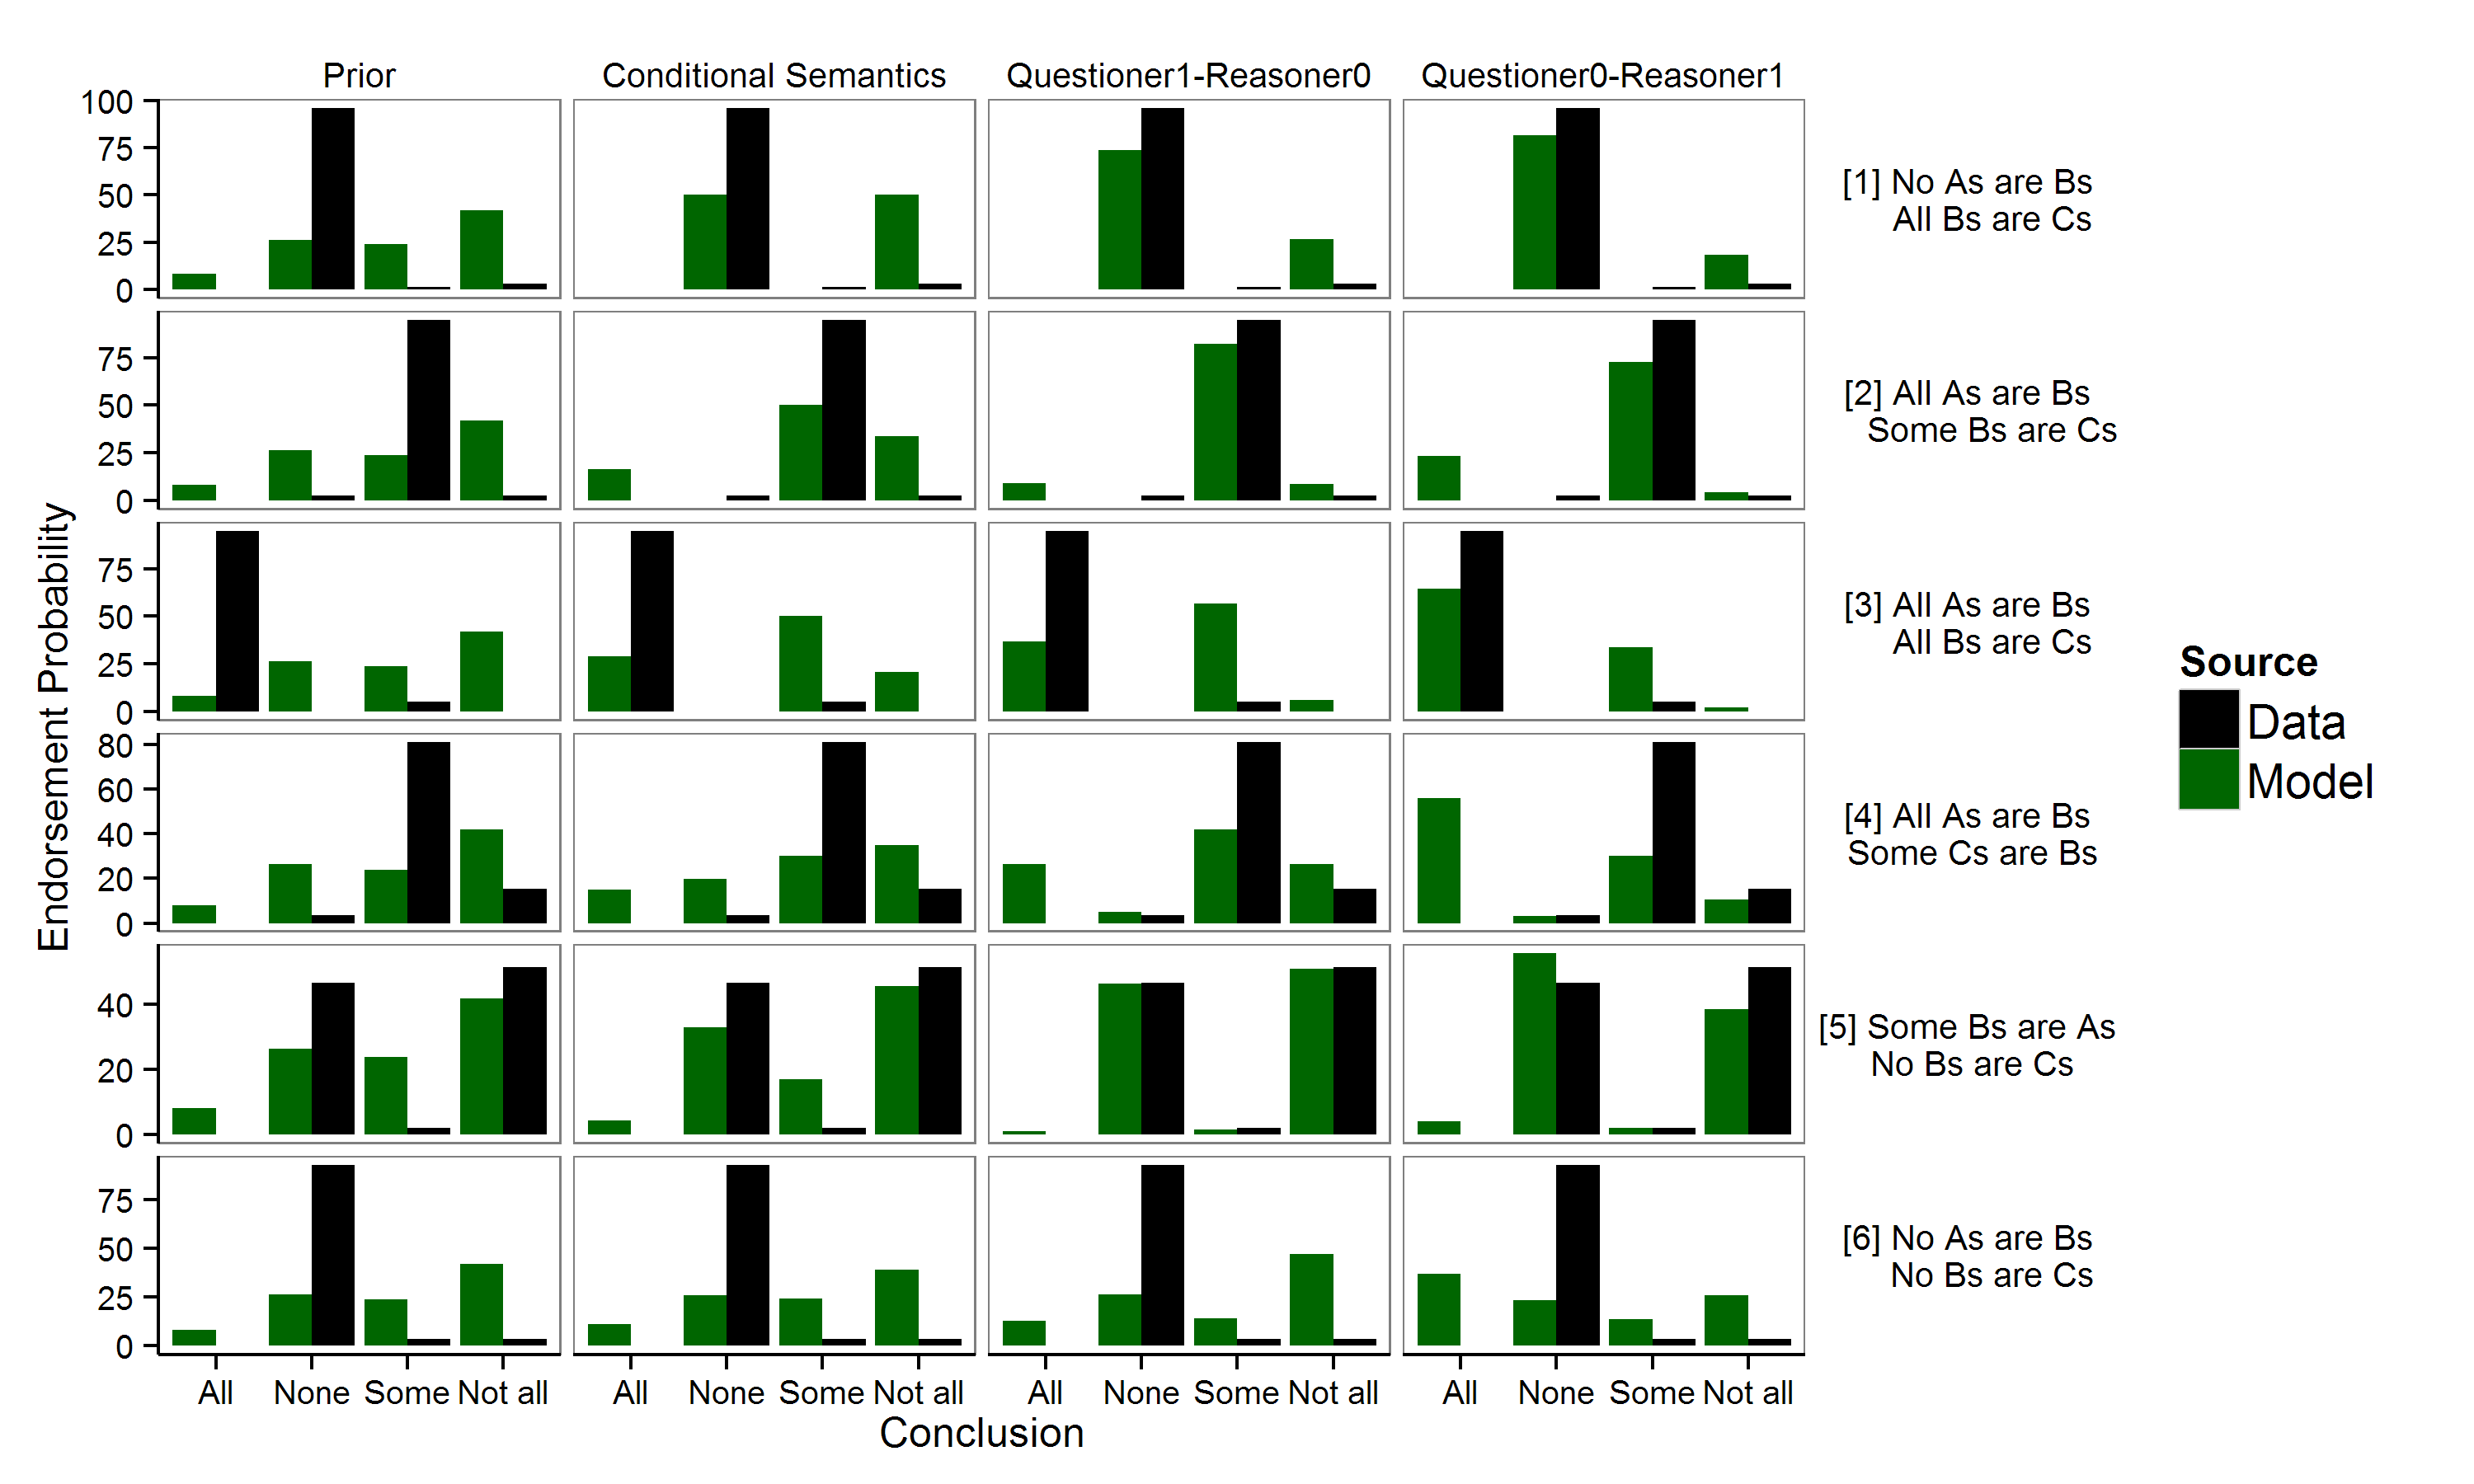
\includegraphics[width=0.9\textwidth,height=8.5cm]{fig1_multibar_qrm_alpha2}
    \caption{Six example syllogisms. 
    [1] Conditional Semantics has no preference among equally valid conclusions; the symmetry is broken by the pragmatics models which uses includes informativity either in its understanding or in its productions.     
    [2] Semantics alone captures the modal response and pragmatics enriches the quantitative fit.     
    [3] The modal response is not as likely in the Semantics model but is a more informative conclusion. [4] Relatively uninformative premises suggest \emph{Some} is the most likely interpretation. [5] Models are able to capture multiple preferred conclusions. [6] Models do poorly in matching subjects' responses in an invalid syllogism.}
  \label{fig:barplots}
\end{figure*}


When we restrict the model to analyzing only situations consistent with the premises being true (the ``literal" reasoner model), the model matches people's maximum judgments on 37 of the 64 syllogisms. The 29 syllogisms for which \emph{not all} was the modal response are qualitatively unaffected i.e. the model matches these responses. As well, the model matches 8 syllogisms for which \emph{some} and \emph{none} are favored (Figure \ref{fig:barplots}, column 2, see e.g. [2]). 

Finally, we introduce pragmatics into the model in both the premise interpretation and the conclusion production sides. We consider first production --- PQR$_{0,1}$. The model is able to distinguish between equally valid conclusions on the basis of informativity (e.g. Figure \ref{fig:barplots} [1], column 4). The model selects not only conclusions likely to be true, but informative (e.g. Figure \ref{fig:barplots} [3]). The model now matches 41 out of 64 modal responses. 

In addition to capturing many of the modal responses, the model is able to accommodate more than one plausible conclusion. Example [5] in Figure \ref{fig:barplots} highlights one such example. This is a syllogism with a valid conclusion but one which people find it difficult to draw. The ``literal reasoner" model tells us why. In many of the possible situations in which the premises are true, a \emph{none} conclusion is true. In addition, \emph{none} is relatively more informative than the valid conclusion -- \emph{not all} -- and so the Questioner-Reasoner Models enforces this symmetry. Notice how this is different from Example [3], in which \emph{all} is less likely than \emph{some} after conditioning\footnote{This may seem surprising as the obvious response is \emph{all}. This is the case because there are two \emph{some} responses which are valid and only one \emph{all} response}. In this example, \emph{all} gets pragmatically strengthened over and above \emph{some} due \emph{all}'s much higher relatively informativeness.  


Conversational pragmatics can also enrich the meaning of the premises given to the reasoner. This is PQR$_{1,0}$. The pragmatics comes in by the reasoner considering -- ``why has the questioner produced these premises given that she may have produced a variety of others?" As a first pass, we consider the alternatives to be the set of all premises of the same term orderings. In the syllogism literature, this ordering is referred to as a syllogism's \emph{figure}. This is tantamount to considering the space of possible quantifiers, keeping the structure of the sentence fixed. Critically, the reasoner does not consider these alternatives with respect to the full state of the world (i.e. the sets A, B and C) but rather only with respect to the QUD (i.e. the sets A and C). 

PQR$_{1,0}$ maximally-prefers the modal response of subjects for 42 out of 64 syllogisms. It picks up on some of the very complex phenomena present in syllogistic reasoning. Example [4] is one such case. The premises considered literally are relatively uninformative. The ``literal" model is very similar to the prior (columns 1 \& 2). In this setup, PQR$_{0,1}$ selects the most informative answer -- \emph{all}. On the contrary, PQR$_{1,0}$ considers the question ``why would the questioner have given these premises" and concludes \emph{some}. Indeed, this is how people reason in this example. 

Still, there are many syllogisms for which reasoning patterns are not accounted for PQR. A large subset of these are syllogisms which use two negative quantifiers (\emph{not all} or \emph{none}). These problems, in a way, are underconstrained in terms of the situations consistent with the premises. For this reason, the models' predictions do not differ appreciably from the prior (Figure \ref{fig:barplots} [6]).

\subsection{Model fit}

To assess our models' quantitative fits we examine correlations across all 256 data points (64 syllogisms x 4 conclusions).

The prior's predictions are the same for all syllogisms and the overall fit is also accordingly poor (r = 0.36) (Figure \ref{fig:megaScatter}, row 2, column 1).  After conditioning on the truth of the premises, the model is able to make graded responses for each of the syllogisms. These responses are a reflection of the types of situations consistent with the premises. The overall correlation is appreciably higher (r = 0.64 (Figure \ref{fig:megaScatter}, row 2, column 2). Among valid conclusions, however, (squares in Figure \ref{fig:megaScatter}) the fit is terrible (r = -0.20). This is a direct consequence of ``literal reasoner"'s literalness. The model has no preference because each valid conclusion is true in every possible situation.

This symmetry is broken by using pragmatic reasoning (Figure \ref{fig:megaScatter}, columns 3-5). The reasoner who interprets the premises as coming from a pragmatic speaker -- PQR$_{1,0}$ -- provides a better fit to the data (column 4, r = 0.69). As well, the model is now able to make graded responses among valid conclusions -- ``the questioner meant for me to infer ..." (r = 0.62). The reasoner who takes the premises at face value but who produces conclusions to be informative provides an even better fit to the data (column 4, r = 0.75). As well, the fit among valid conclusions -- ``\emph{all} is a better conclusion than \emph{some}" -- is even stronger (r = 0.82). 

PQR$_{1,1}$ -- which reasons pragmatically on both the production and the interpretation -- does not model the data any better than the individual processes. This joint model selects the modal response on 41 out of the 64 syllogisms and provides a worse fir than either of the individual PQR models (r = 0.66). This is likely do to the particular way in which the information between the two inference processes is shared. We leave for later work the proper way of combining information between the avenues of pragmatic inference.


%We compared these results to those found when using a uniform prior (\ref{fig:megaScatter}, row 1)) and found the overall fit much better with the binomial, which invokes the principle of rarity. 

\begin{figure*}[t!] %[htp]
\centering
	\subfigure
		\centering
  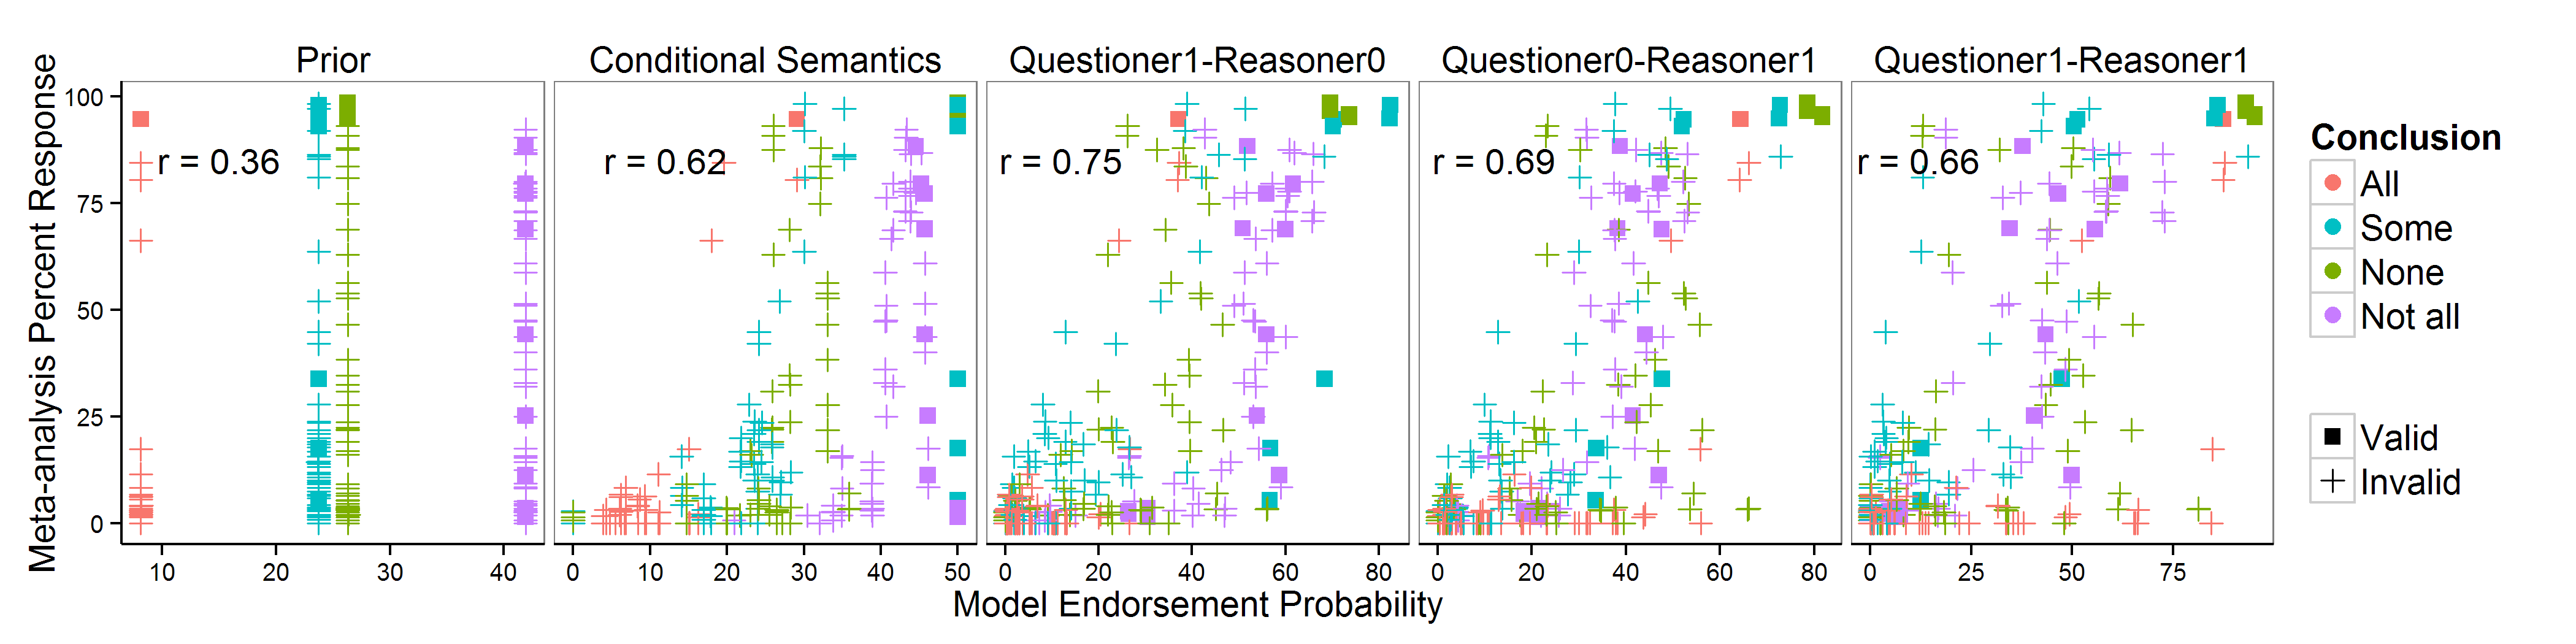
\includegraphics[width=\textwidth,height=4cm]{fig2_multiScatter_qr5_n6_alpha2}
  \caption{Human subject percentage endorsement vs. model fits.
  Columns (from L to R): predictions based only on the prior, Conditional Semantics models, and Questioner-Reasoner models. The number {0,1} next to questioner and reasoner denotes the depth of recursion for interpretation of premises and production of conclusions, respectively.}
  \label{fig:megaScatter}

\end{figure*}

%\subsection{Dependency}



%Using the correlated prior, the Conditional Semantics model gets 45 out of 64 modal responses. The overall fit is also improved, r = 0.75 (Figure \ref{fig:megaScatter}, row 3). The Conditional Pragmatics model does better as well, predicted the modal response for 52 syllogisms. Additionally, the quantitative fit is high (r = 0.85). Among valid syllogisms, it is correspondingly higher as well (r = 0.88). 


\section{Most and few}

Our model is based on a truth-functional semantics and as such, it is able to accommodate any quantified sentence with a truth-functional meaning. The question of the meaning of generalized quantifiers like ``most" and ``few" is a topic of great interest to the field of formal semantics. Often, ``most" and ``few" are modeled by a thresholded step function. As a first test of the generality of the model, we define most and few by a threshold of 0.5 such that ``most As are Bs" is true if more than half of the As are Bs. We realize this is a gross oversimplification of the meanings of these words. We maintain the set size parameter of 6. However, we feel the usage of the words ``most" and ``few" might bias people to represent sets of larger size.

We compare our model predictions to two studies carried out by \Acite{Chater1999} on syllogisms using the generalized quantifiers \emph{most} and \emph{few} e.g. \emph{Most artists are beekeepers. Few chemists are beekeepers.}. Participants were told to indicate which, if any, of the four quantifier conclusions followed from the premises and were allowed to select multiple options.

The set of all possible syllogisms with 6 quantifiers is 144 questions.  The authors divided these into two experiments to avoid subject fatigue. Experiment One consisted of the \emph{all},\emph{not all},\emph{most}, and \emph{few} quantifiers. Experiment Two used \emph{most},\emph{few},\emph{some}, and \emph{none}. 

\begin{figure*}[t]
	\centering
  \includegraphics[width=\textwidth]{fig3_multiScatter_AMFO_MFIE_n6_alpha2}
      \caption{Human subject percentage endorsement vs. model fits for 2 experiments using generalized quantifiers. Experiment 1 (left) used the quantifiers \{\emph{all}, \emph{most}, \emph{few}, \emph{not all}\}. Experiment 2 (right) used the quantifiers \{\emph{most}, \emph{few}, \emph{some}, \emph{not all}\}.}
  \label{fig:mfScatter}
\end{figure*}


We find good correspondence between the experimental data and the model, even without further parameter fitting (Figure \ref{fig:mfScatter}). In Experiment 1, the quantifiers \emph{all}, \emph{most}, \emph{few}, and \emph{not all} were used. The PQR$_{0,0}$ model selected the modal response for 45 out of 64 syllogisms and had a good quantitative fit (r = 0.79).  PQR$_{1,0}$ selected 48 modal responses and had an even better quantitative fit (r = 0.81). PQR$_{0,1}$ selected 50 modal responses and had a slightly worse fit (r = 0.76). 

In Experiment 2, the quantifiers \emph{most},\emph{few},\emph{some}, and \emph{none} were used. PQR$_{0,0}$ selected the modal response for 34 out of 64 syllogisms and had a correlation of r = 0.63. PQR$_{1,0}$ selected 43 modal responses with  r = 0.63. PQR$_{0,1}$ selected 44 modal responses and had a slightly worse fit r = 0.60. 

The fit is appreciably better for Experiment 1 than for Experiment 2. The same was true for the Probability Heuristics Model (r = 0.94 vs r = 0.63). Overall, the proportion of \emph{no valid conclusion} responses in the experimental data, which we do not model, was much higher in Experiment 2 than in Experiment 1. This data set may well contain more noise in the measures we model than the others discussed in this article. 

\section{Relationship to previous theories}

A recent meta-analysis carved the space of reasoning theories into three partitions: those based on models or diagrammatic reasoning, those based on formal logical rules, and those based on heuristics \cite{Khemlani2012}. We see the space slightly differently. In one dimension, theories may be based on applying propositions -- be they heuristic or logical -- or they are based on constructing concrete representations or models. In another dimension, theories may be considered fundamentally probabilistic or deterministic. 

We now review 2 theories which we take to exemplify two of the four quadrants of this theoretical space. 

\subsection{Mental Models}
 The Mental Models Theory (MMT) describes a psychological process by which people reason by constructing {\em iconic} mental representations or models, which represent the terms of a proposition as a collection of individuals. In syllogistic reasoning, a model is constructed for each premise, and premise models are consolidated so that the conclusion may be ``read off" the joint model. For example, a model for the premise  \emph{All colleagues have the flu} could be represented as the following situation.

\begin{tabular}{l l}
colleague & flu\\
colleague & flu\\
 & flu\\
\end{tabular}

This shows 2 individuals who are colleagues and have the flu, and one individual who is not a colleague and has the flu. Thus, each row is a representation of the properties of an individual. MMT emphasizes the need to search for counter-examples to check for logical validity. Errors arise in this search process. Another premise might read: \emph{Some people with the flu are out for weeks}. This would look like:

\begin{tabular}{l l}
flu & out for weeks\\
flu & \{out for weeks\}\\
 & \{out for weeks\}\\
\end{tabular}

The curly brackets reflect the fact that multiple distinct models could be drawn in accord with this premise. Conclusions are achieved by consolidating these models and reasoning over the joint model. Thus, a reasoner would have to construct all possible distinct models in order to determine that no proposition is true in all of them. 

The MMT captures the intuition that people are able to reason about sets of things explicitly and with respect to context. At the same time, the theory is not well defined insofar as it does not specify \emph{how} various models come into existence, only that various models \emph{can} come into existence. Mental models are very similar to the \emph{situations} described in the Probabilistic Questioner-Reasoner model. A critical difference is that in PQR, situations are constructed by sampling. Thus, PQR can make quantitative predictions about reasoning patterns with no further assumptions. 

Finally, the \emph{a priori} believability of propositions has been shown to have an important effect on reasoning \cite{Oakhill1989}. Mental models are flexible in that content can motivate one to carry on the search process longer. We assumed in this article that PQR samples from an independent prior. This is likely not the case when content affects reasoning. PQR is able to make this notion of context-sensitivity explicit by incorporating background knowledge into the prior from which situations are sampled. 

%Different quantifiers can be applied by reasoning over these mental models; indeed one just needs to ``read off" the model to see if a certain proposition is true. Thus, it has been proposed that mental models could account for usage of generalized quantifiers (e.g. most and few) in syllogistic reasoning, though this claim has not been substantiated by empirical work or a model.

%\subsection{Mental Logics}
%
%Rips (1994) proposed that people reason according to rules of \emph{natural deduction}. The theory of Mental Logics, instantiated in the PSYCOP model, posits individuals construct \emph{logical sentences} in a language of first-order predicate calculus which are linked when the ``individual recognizes [the link or inference] as intuitively sound". The model explains errors as a failure to recognize the applicability of a given formal rule, a failure to retrieve the rule, or a failure to carry out the necessary steps for that rule. People are especially prone to such errors when complex rules are needed so there is a predicted effect of rule complexity on difficulty. In this instance, the theory does not specify \emph{which} conclusions will be drawn fallaciously, only that some will. Mental Logics posits that people reason according to logical, deterministic rules. 

\subsection{Probability Heuristics}

\citeA{Chater1999} introduced the Probability Heuristic Model (PHM) as an attempt to capture the intuition that people are using \emph{everyday} reasoning when asked to resolve syllogisms. To accomplish this, the PHM lays out a computational level theory which includes an ordering of propositional informativity, a probabilistic semantics, and a probabilistic notion of validity. The PHM derives its informativity ordering at the propositional level by assuming categories are represented as hyperspheres in a high-dimensional concept space. Our model takes a different approach. PQR uses a truth-functional semantics which it applies to samples from a distribution over situations. An ordering of informativity emerges from the fact that all quantified propositions are not equally likely across situations.

The PHM relies on a number of {\em generation} and {\em test} heuristics to produce and quantify confidence in conclusions. We do not believe these heuristics are necessary for deriving a probabilistic model of reasoning. Further, the very nature of their heuristics suggests reasoners are engaging with the syllogisms at a propositional level and not at the level of concrete representations. We consider heuristic accounts analogous to formal rule theories (e.g. \citeA{rips1994}) in that people are reasoning at the level of propositions, which in the case of the PHM, are determined by probabilities. We also do not believe this to be the case.

\section{Discussion}

The theoretical partitioning described above places the Probabilistic Questioner-Reasoner model in a previously unexplored quadrant of the two-dimensional theoretical space described: we consider reasoning over concrete situations and situations to be constructed probabilistically by sampling.

We have presented a formal model of syllogistic reasoning based on the \emph{Rational Speech-act} framework. This formalizes the notion that reasoners construct mental situations by sampling and reasoning over these situations, much like has been described in the Mental Models literature. Unlike Mental Models, however, PQR is inherently probabilistic and thus assumes reasoners are in some way gaging degrees of plausibility in syllogistic reasoning tasks. Further, PQR is fundamentally quantitative, and thus can be considered an elaboration of the Mental Models theory.

The inspiration for this model comes from the idea that syllogistic reasoning can not be disentangled from language understanding. In particular, natural language semantics is insufficient to explain the variability in such a data set. We argue that understanding conversational pragmatics is necessary to understanding how people reason with syllogistic arguments. We have found that the meanings of quantifiers are important insofar as \emph{some} might imply \emph{not all} and so people prefer to conclude \emph{all} when it is warranted. 

This is early work and we have found promising evidence, both qualitative and quantitative, that this framework will allow for a more explicit understanding of syllogistic reasoning. As well, this model is flexible enough to capture some of the variability in reasoning data using generalized quantifiers. We tested the model assuming a naive threshold of 0.50, such that \emph{most} is true if more than half is satisfied. We don't believe these quantifiers are modeled perfectly in this way, and we will explore more context-sensitive formulations in future work.

In this framework, a syllogism is read as an argument given as a part of discourse between people. Indeed, this is how syllogisms were used in the time of Aristotle and in the long tradition of scholastic philosophers. Fundamentally, syllogisms are a tool used to convince others. The results of the Questioner-Reasoner models shed light on the idea that human reasoning behavior in the syllogistic task is as much reason as it is human. Gaging degrees of plausibility alone is not sufficient. A listener needs to be posited at the end of the line so that a conclusion makes sense; so that a conclusion is convincing!

If one accepts that the purpose of a syllogism is to convince, a natural question arises. Why not just assert ``Some of my colleagues won't be at work for weeks" from the get-go? Why go through the trouble of laying out premises and having a person draw the conclusion? Arguments are used to persuade, and not all assertions are equally believable \emph{a priori}. The reason premises are presented in this way is that there is no reason to believe some  colleagues will be out of work for weeks. That only happens around Christmas. And so the conclusion is not obvious, and the premises are an alternative route to persuasion. If we accept the premises, we are left with no choice but to draw the conclusion.

We set out to explore this intuition by seeing if considering alternatives in the interpretation of premises would better account for the data than a literal interpretation of premises. We did this not in the context of the true state of the world but with respect to the QUD. Thus, pragmatic interpretation is different from standard Gricean implicatures. We found this to be important in capturing human reasoning patterns.

The two Questioner-Reasoner models presented interact in complex and yet not well understood ways. Individually, they account for much of the data, and in non-overlapping ways. The number of syllogisms whose modal response was not predicted by either model is a mere 9 (i.e. 55 out of 64 syllogisms were accounted for by one of the models). This suggests some complex interaction between pragmatic interpretation of premises and production of conclusions is at work. 


%The rationale is that if someone is to go through the trouble of mentioning the middle term, it must allow them to assert something that they wouldn't be able to assert otherwise. In other words, we speculate the \emph{a priori} probability of A \& C is taken to be relatively low, but may become higher if B is observed. In this way, A \& C become correlated via B. This is akin to saying that the end terms have a special relationship via the middle term. It is no coincidence that the middle term appears in both premises and it is no coincidence the premises appear at all. 

%We modified the naive binomial prior to induce a slight correlation between A \& C via B. Overall, the model matches a few more modal responses and provides a better quantitative fit to the data. However, we do not assert that the probability of co-occurrence to be \emph{a priori} unlikely in the case of syllogistic reasoning tasks. Many of the experimental materials in the meta-analysis data were well controlled for semantic content. Rather, we see this as arising from conversational pragmatics. It is a future direction of this work to develop a formal model of this phenomenon.

%\end{figure*}}
%\subfigure[prior]{ %
%	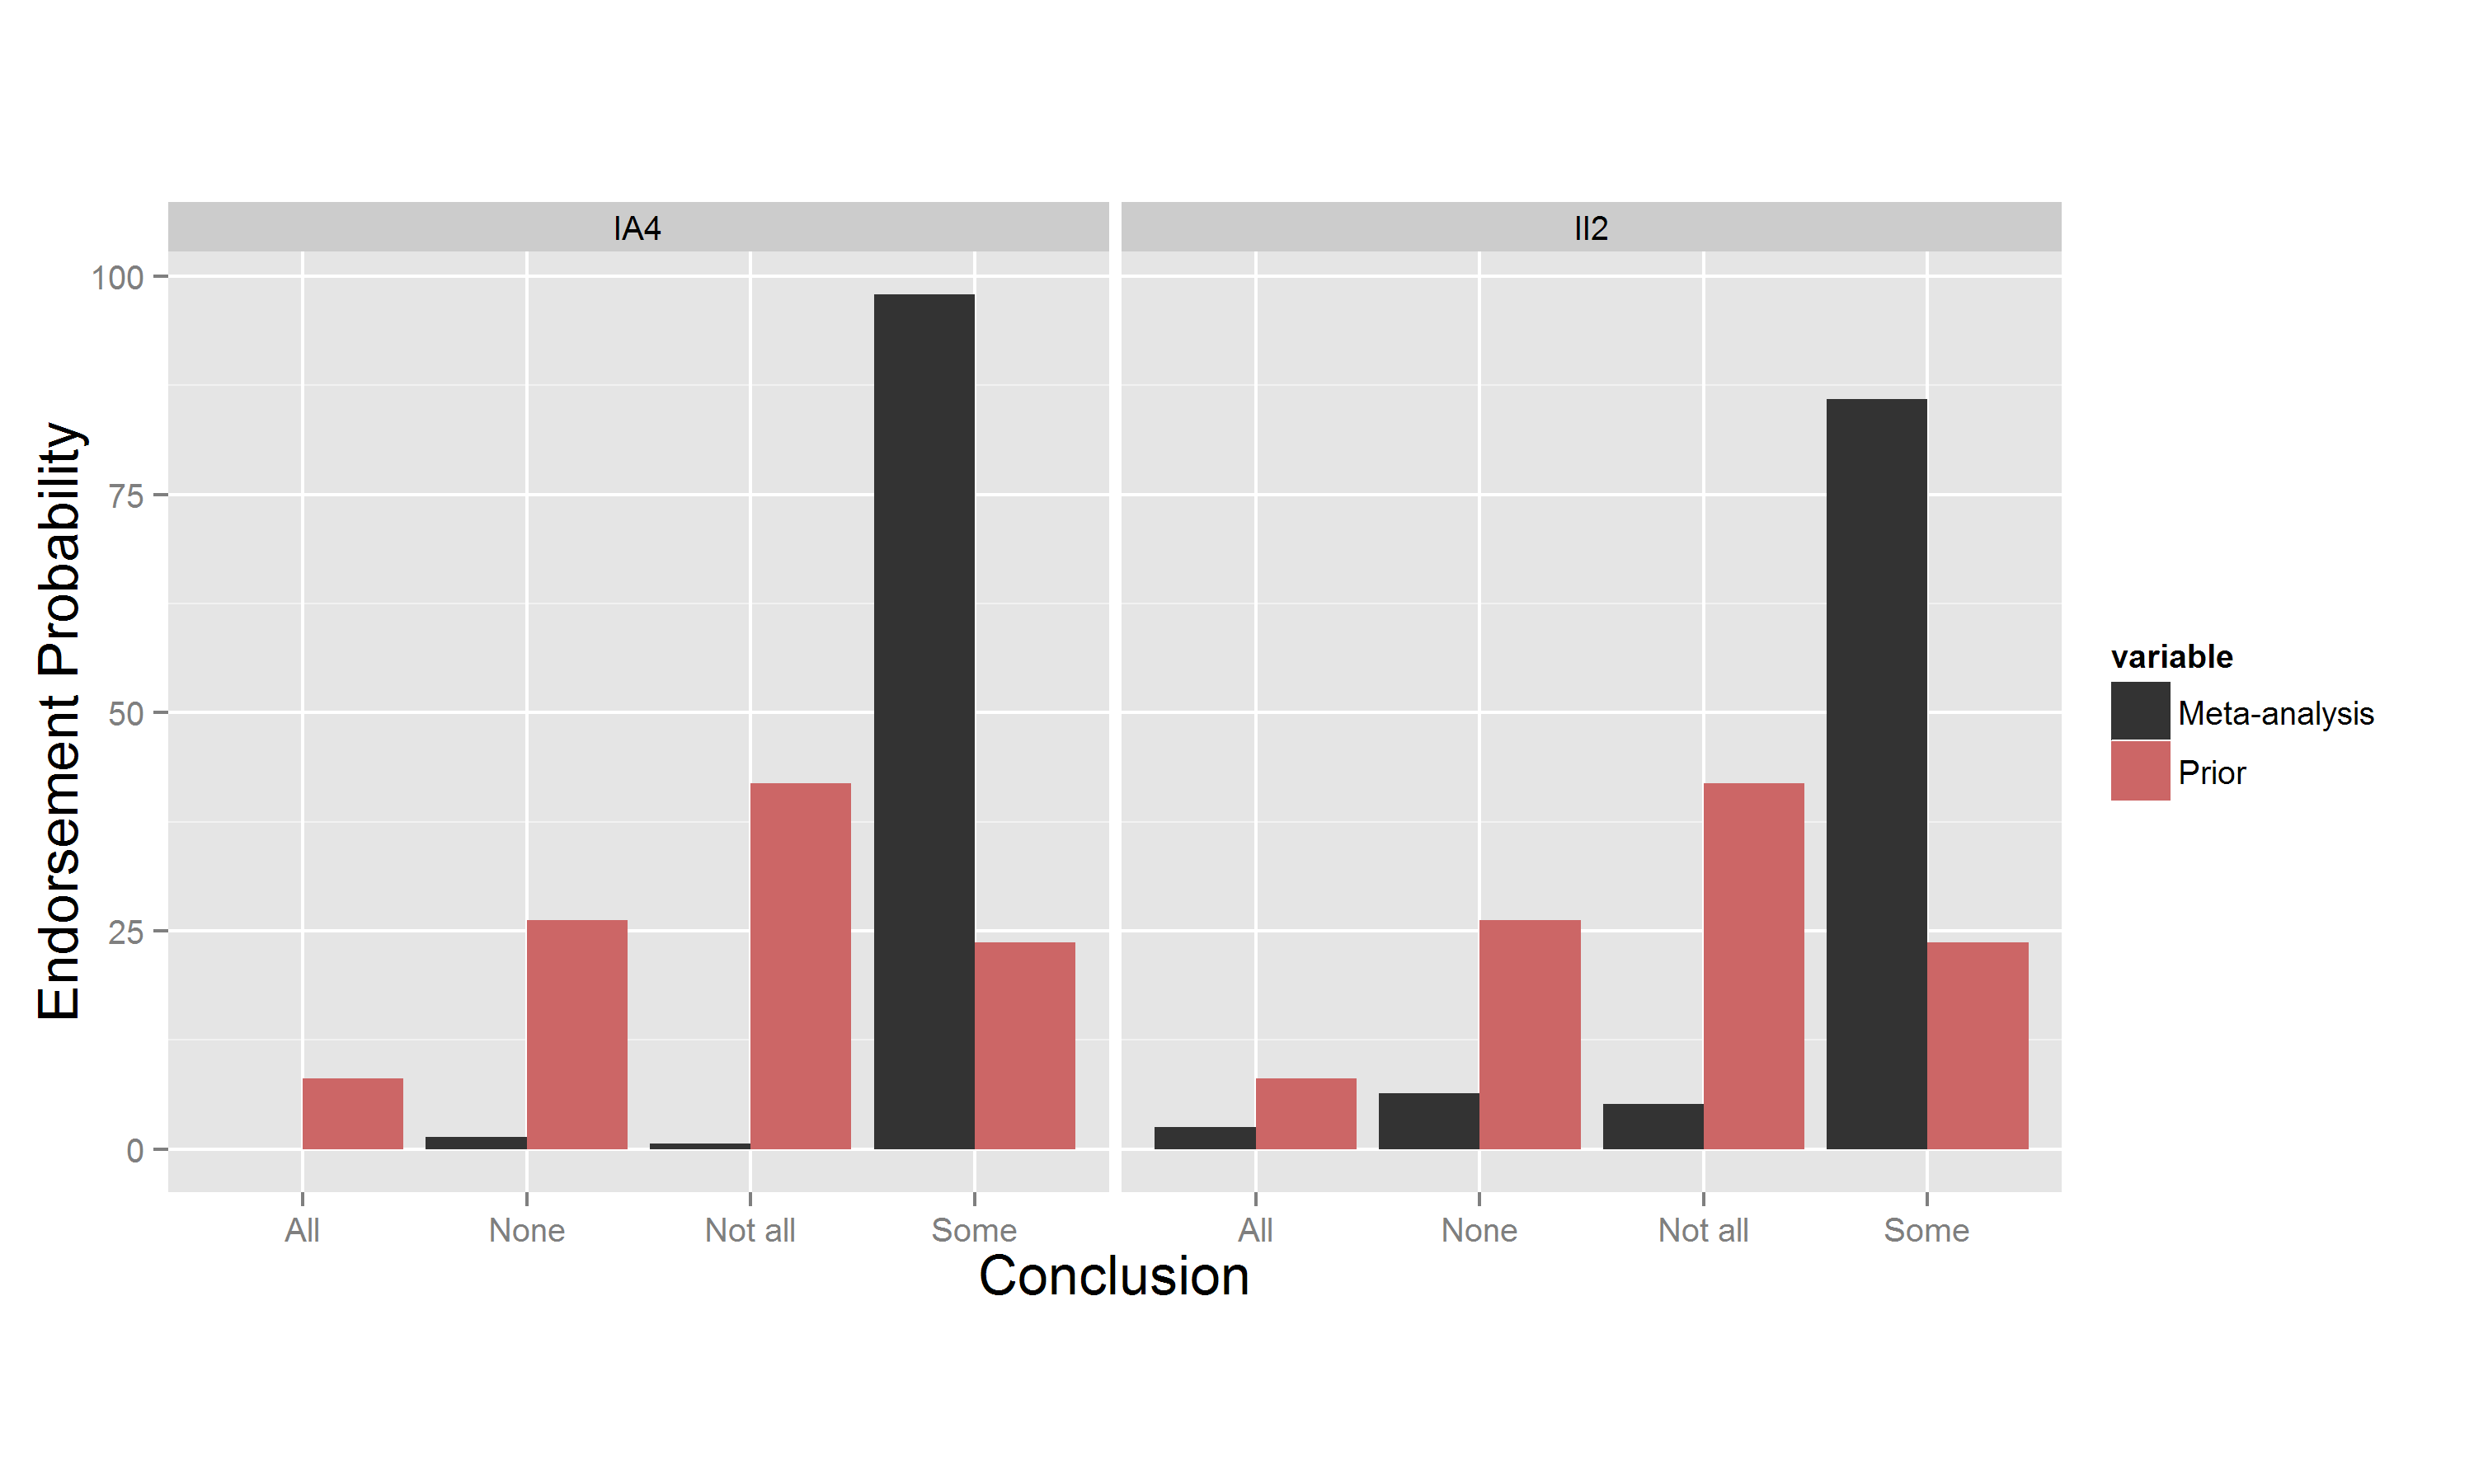
\includegraphics[width = {0.66\columnwidth}]{multibar_alpha1_prior}
%	\label{fig:subfigure1}}
%%\caption{Single-model, valid}}
%%\hfill
%\subfigure[conditional semantics]{ %}
%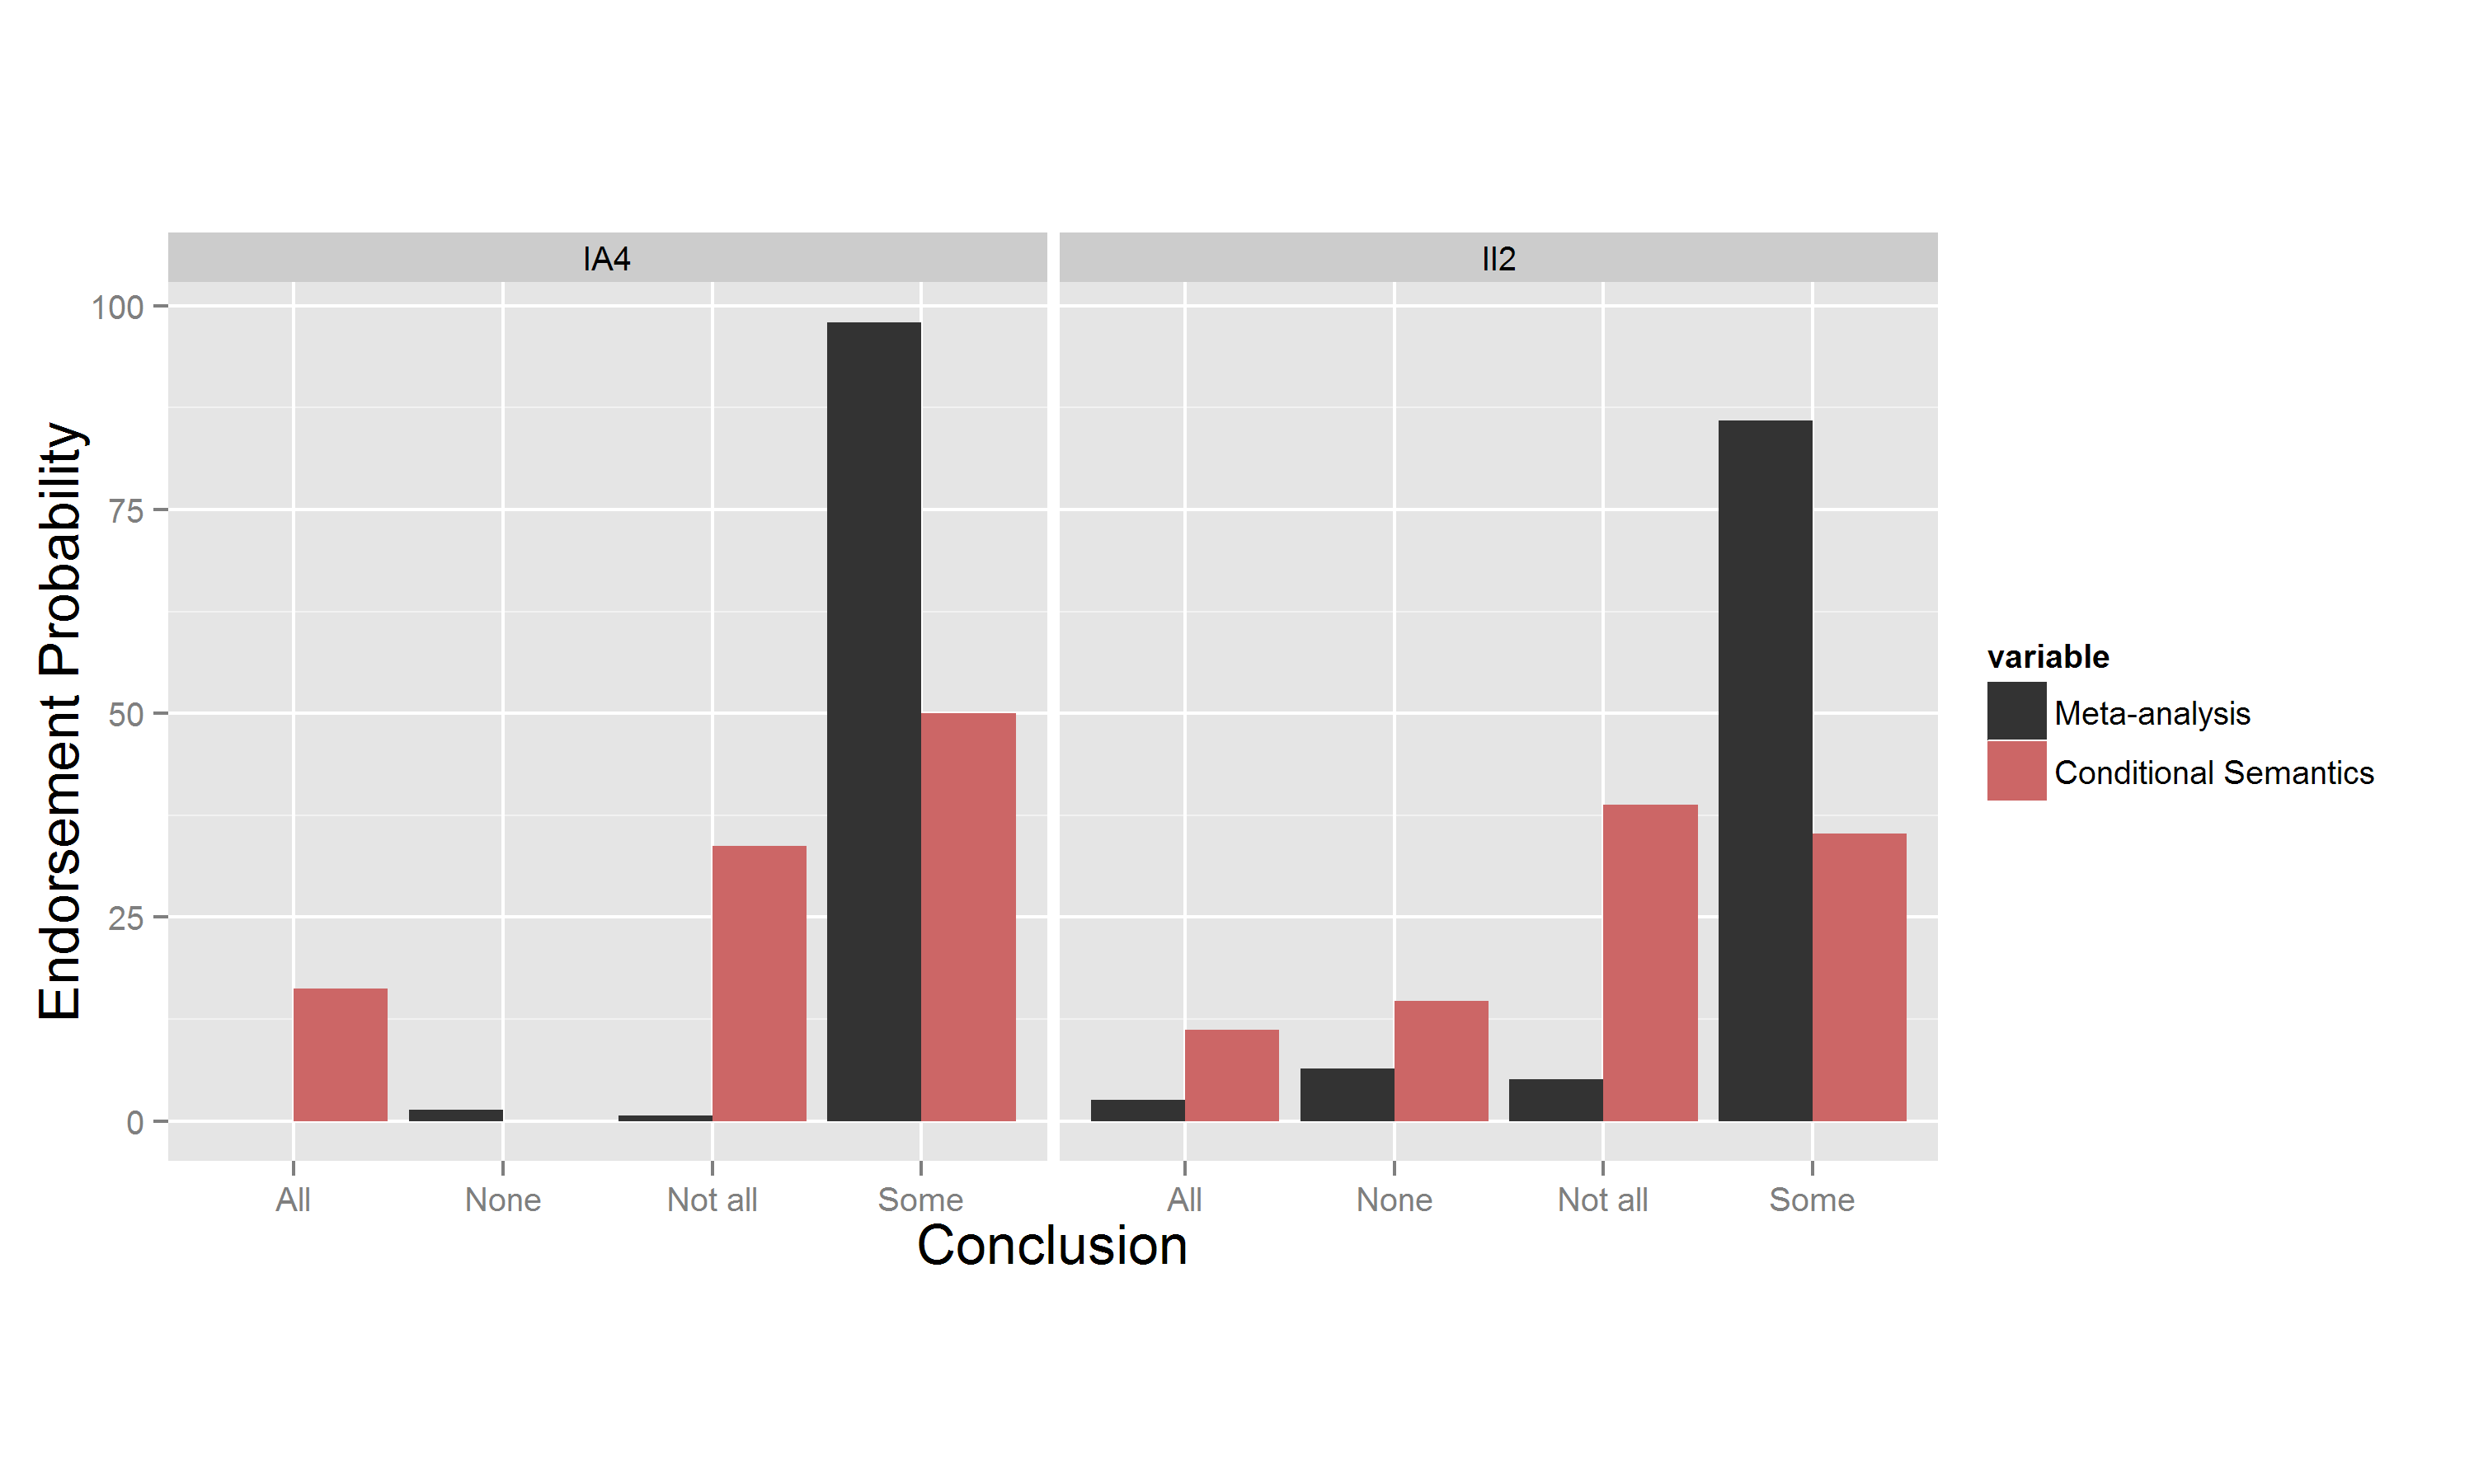
\includegraphics[width = {0.66\columnwidth}]{multibar_alpha1_lit}
%%\label{fig:subfigure3}
%\caption{Multiple-model, valid}
%}
%%\hfill
%\subfigure[conditional pragmatics]{
%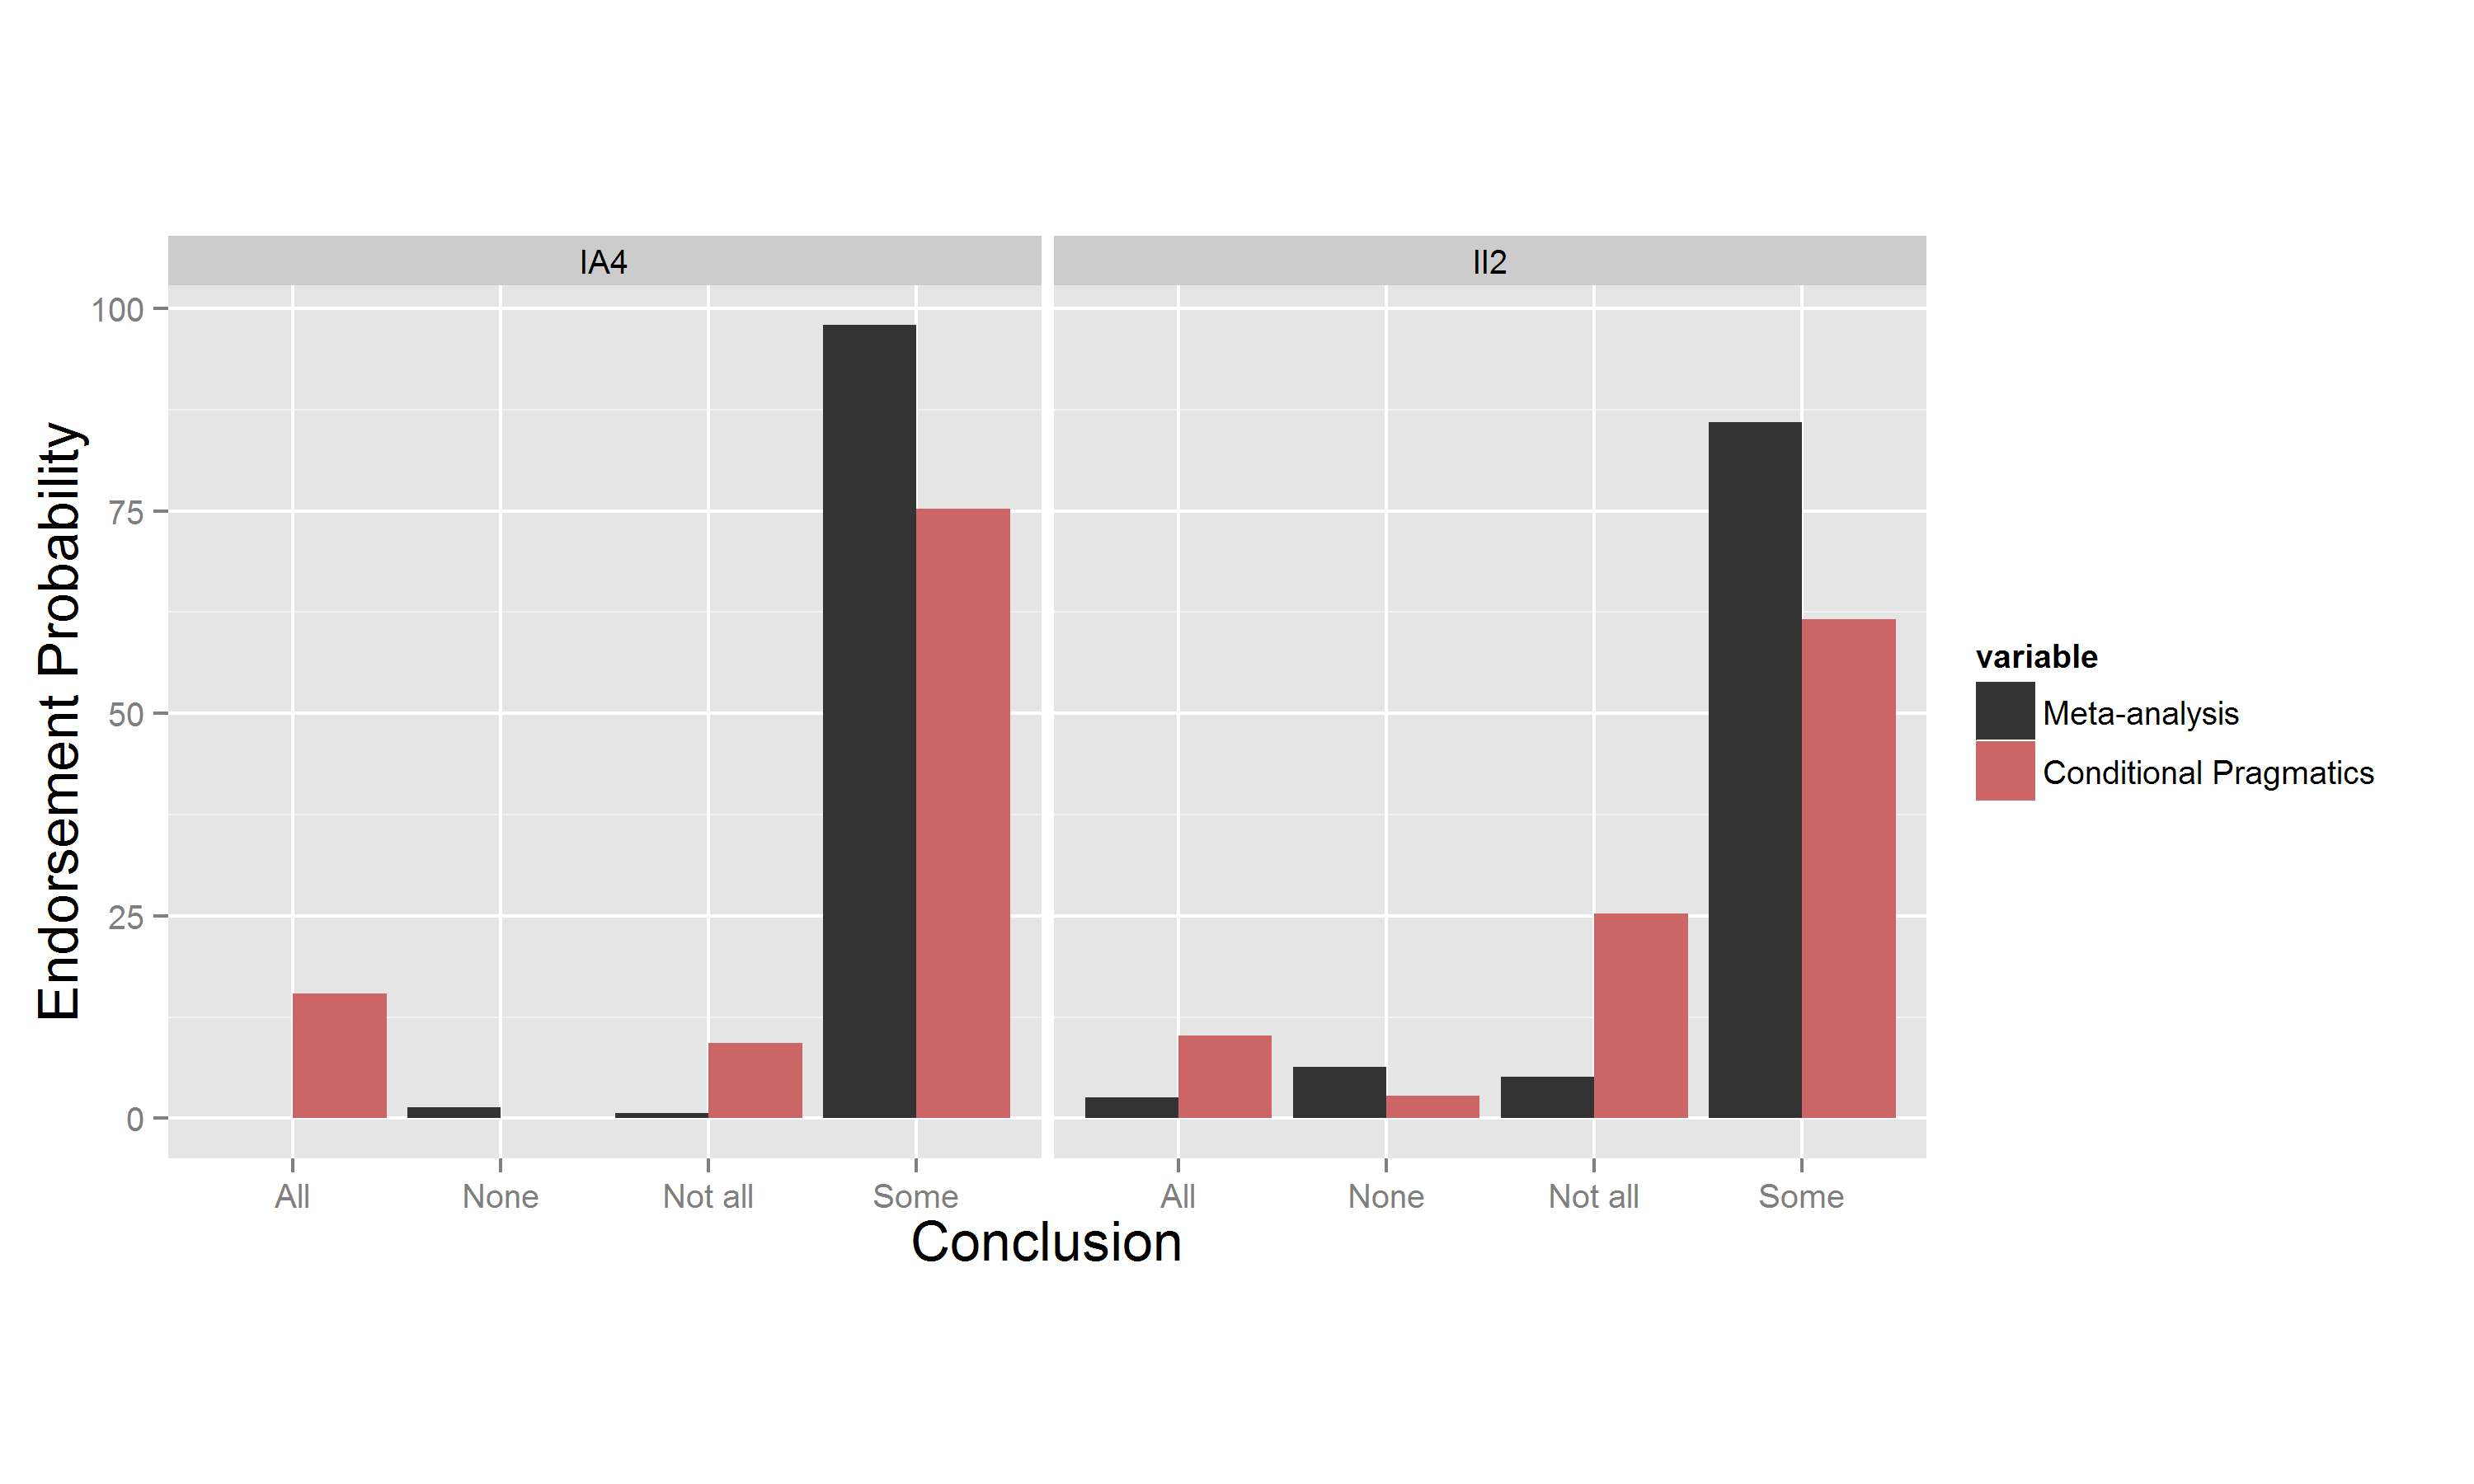
\includegraphics[width = {0.66\columnwidth}]{multibar_alpha1_prag}
%%\label{fig:subfigure5}
%\caption{invalid}
%%}
%%\quad
%%
%%\subfigure[one model, valid]{ %
%%\includegraphics[width = {0.66\columnwidth}]{IA4_boxplot_text}
%%%\label{fig:subfigure2}}
%%\hfill
%%\subfigure[multiple models, valid]{
%%\includegraphics[width = {0.66\columnwidth}]{EI3_boxplot_text}
%%%\label{fig:subfigure4}}
%%\caption{Multiple-model, valid}
%%\hfill
%%\subfigure[invalid]{
%%\includegraphics[width = {0.66\columnwidth}]{AA2_boxplot_text}
%%%\label{fig:subfigure6}}
%%\caption{invalid}
%%
%%\caption{Participants' endorsements in six syllogisms}
%%\label{fig:fig1}


%
%
%Mental Models Theory explains difficulty in syllogisms by demonstrating that multiple, distinct situations can be consistent with a pair of premises, giving rise to different possible conclusions. Valid syllogistic conclusions arise in every possible model. (This is the same notion of Pr(conclusion | premises) = 1). 
%
%This is always the case the logically invalid syllogisms (see discussion below), and is sometimes the case with logically valid syllogisms.

%\subsubsection{Logical invalidity}
%For syllogisms that have no valid conclusion, the probabilistic reasoner computes the probability of the conclusion conditioned on the premises being true by sampling. For all invalid syllogisms, this yield a gradeds response across the different possible conclusion types. 
%
%
%\subsubsection{Logical validity}
%A conclusion is logically valid if and if only it is true in all possible situations. Recall that possible situations are restricted to those that are consistent with the premises. The universal quantifiers (all, none) entail their particular counterparts (some, not-all), respectively. This was noticed by Aristotle and commonly visualized in the \emph{Square of Opposition}. For our probabilistic reasoner, confidence for {\emph all} and {\emph some} (to take the affirmative case) will be both maximal. {\emph All} is always true and {\emph some} is true whenever {\emph all} is true.


%We tested a number of rarity factors and found that p=0.25 provided the best fit. This is also consistent with the Probability Heuristic's rarity assumption. 


%\red{math here?}

%For reasoning over syllogisms, the prior distribution is conditioned on the truth of the premise sentences. This is the distribution over sentences conditioned on the fact that the premises are true. In this way, we evaluate the $\Pr$(conclusion $\arrowvert$ premises). This is essentially a metric of the plausibility of the argument. In this formulation, $\Pr$(conclusion $\arrowvert$ premises) = 1 if and only if the syllogism is logically valid.

%
%To set this parameter, we follow Johnson-Laird's principle of parsimony, which states that situations are constructed to ``maximize the number of properties of each individual to try to keep the number of \emph{distinct sorts} of individuals to a minimum".
%
%, from which we accept only those consistent with the premises \footnote{We follow J-L's lead by imposing the additionasl constraint that the syllogistic terms refer to non-empty classes in the world. This is the existential presupposition.}.
%
%The basic model has two parameters, which both contribute to the concept of Expected Value: situation size and property rarity. We tested a number of situation sizes and found 6 to be the best. This is consistent with Johnson-Laird's principle of parsimony which states that models are constructed to ``maximize the number of properties of each individual to try to keep the number of \emph{distinct sorts} of individuals to a minimum". 
%
%The number of distinct sorts of individuals is highest for logically invalid syllogisms precisely because the problems are not fully constrained. In Johnson-Laird's examples of these types of models, the number of individuals is always 6. 
%
%Rarity refers to the probability that a particular object in a world has a property (or belongs to class). A principle of rarity is often assumed in line with the intuition that properties are relative rare \footnote{This article is an article and it's about reasoning, but it's not a cat, and it's not a car, nor an elephant nor the color red. In fact, there's a very large number of things which this article is not.}, and we assume a principle of rarity here. We tested a number of rarity factors and found that p=0.25 provided the best fit. This is also consistent with Chater \& Oaksford's rarity assumption. 

%\subsection{Model predictions}

\

\bibliographystyle{apacite}

\setlength{\bibleftmargin}{.125in}`
\setlength{\bibindent}{-\bibleftmargin}

\bibliography{mhtbib}


\end{document}



TODO after cogsci:
-implement phm (and mm?) for comparison.
-understand alpha param and pragmatic production recursion depth.
-understand the origin of symmetry breaking in 'prior' (i.e. funny prior which should be pragmatic).
-understand why pragmatic comprehender model doesn't work.
-analyze errors better.
-do experiments to get estimate of priors.
